\section{Ingesta de datos}\label{sec:impl_ingesta}
Tras la creación y el despliegue de la infraestructura base, se procede a la
creación de los scripts de ingesta de datos, de manera escalonada y siguiendo
la prioridad de las fuentes de datos.

Esta sección de la memoria documenta el desarrollo de las siguientes historias
de usuario, siguiendo la planificación establecida en la sección \fullref{sec:planif_inicial}:

\begin{table}[H]
	\centering
	\begin{tabular}{|p{0.7\linewidth}|c|c|}
		\hline
		\textbf{Nombre} & \textbf{Prioridad} & \textbf{Tamaño} \\
		\hline
		\hline
		Como desarrollador de Okticket, quiero que se ingesten de manera automática datos de la base de datos interna de MongoDB & P0\cellcolor{red!50} & M\cellcolor{yellow!50} \\
		\hline
		Como desarrollador de Okticket, quiero que se ingesten de manera automática datos de la base de datos interna de MySQL & P0\cellcolor{red!50} & M\cellcolor{yellow!50} \\
		\hline
		Como desarrollador de Okticket, quiero que los datos se limpien de manera automática & P0\cellcolor{red!50} & S\cellcolor{green!25} \\
		\hline
		Como desarrollador de Okticket, quiero que se ingesten de manera automática logs de balanceador de AWS & P1\cellcolor{orange!50} & M\cellcolor{yellow!50} \\
		\hline
  \end{tabular}
  \caption{Lista de HUs cumplimentadas con la ingesta de datos}
  \label{tab:impl_ingesta}
\end{table}


\newpage{}
\subsection{Ingesta de métricas con Kafka}\label{subsec:impl_ingesta_kafka}
Puesto que se ha decidido utilizar Kafka como sistema de mensajería, se
desarrollan los scripts de ingesta de datos para que los datos se envíen a
Kafka y se procesen mediante Logstash y Elasticsearch.

Para la ingesta de datos, se han desarrollado scripts de Python que se encargan
de la lectura de los datos de las fuentes, su transformación y su envío a Kafka.
Estos scripts se ejecutan en bucle con una parada de segundos entre ejecuciones,
aunque se pueden adaptar para cualquier otra ejecución periódica como triggers,
\textit{cron jobs} o \textit{webhooks}.

Algunos de los servidores que contienen la información a ingestar se encuentran
detrás de subredes privadas, por lo que los scripts de ingesta se deben ejecutar
a través de \texttt{SSH} en los servidores bastiones de dichas subredes. Estos
servidores se encargarán de conectar con la infraestructura desplegada y enviar
la información.

\textit{Ver código: \fullref{anexo:kafka}}


\subsubsection{Componentes de Kafka}
\textit{Kafka} se compone de varios componentes clave:

\begin{itemize}
    \item \textbf{Tópico}: Un tópico es una categoría a la que se envían los
		mensajes y a la que los consumidores están \textit{suscritos}. Los
		consumidores pueden estar suscritos a uno o varios tópicos, y los
		productores pueden enviar mensajes a uno o varios tópicos. Los tópicos
		son la unidad básica de organización de los mensajes en cualquier
		sistema de mensajería de publicación/suscripción.
    \item \textbf{Productor}: El productor es el componente responsable de crear
		y enviar mensajes al cluster de Kafka. Está separado del resto de los
		componentes y produce mensajes de manera asíncrona y rápida.
    \item \textbf{Consumidor}: El consumidor es el componente responsable de
		leer los mensajes producidos por el productor. Está suscrito a un tópico
		a través del broker y consume los mensajes.
    \item \textbf{Broker}: El broker es el componente responsable de recibir los
		mensajes producidos por el productor y enviarlos a los consumidores. Es
		el intermediario entre los productores y los consumidores.
\end{itemize}


\newpage{}
\subsubsection{Explicación del código}
Todos los \textit{productores} de datos siguen un patrón similar, ya que su
función es la misma: leer datos de una fuente, transformarlos y enviarlos a
Kafka.

Su código se divide en tres partes principales, siguiendo con el patrón de
diseño de \textit{Extract, Transform, Load} (ETL) definido anteriormente
(ver~\ref{sec:etl}):

\begin{itemize}
	\item \textbf{Lectura de datos:} se encarga de la lectura de los datos de
		la fuente de datos. En el caso de las bases de datos, se conecta a la
		base de datos y ejecuta una consulta para obtener los datos. En el caso
		de los logs, se lee el fichero de logs y se extraen las líneas que
		contienen la información necesaria.
	\item \textbf{Transformación de datos:} se encarga de la transformación de
		los datos leídos a un formato adecuado para su envío a Kafka. En el caso
		de las bases de datos, se transforman los datos a un formato JSON. En el
		caso de los logs, se transforman las líneas de logs a un formato JSON.
	\item \textbf{Envío de datos:} se encarga del envío de los datos a Kafka.
		Para ello, se conecta a Kafka y envía los datos a un tópico concreto.
\end{itemize}


\subsubsection{Dependencias}
Para la ejecución de los scripts de Python, se necesitan las siguientes
librerías, dependiendo del script a ejecutar:

\begin{itemize}
	\item \textbf{kafka-python:} librería de Python que permite la conexión y
		el envío de datos a Kafka.
	\item \textbf{pymsql:} librería de Python que permite la conexión y la
		ejecución de consultas en bases de datos MySQL.
	\item \textbf{pymongo:} librería de Python que permite la conexión y la
		ejecución de consultas en bases de datos MongoDB.
	\item \textbf{python-dotenv:} librería de Python que permite la carga de
		variables de entorno desde un fichero \texttt{.env}.
\end{itemize}


\newpage{}
\subsection{Ingesta de logs de AWS}\label{subsec:impl_ingesta_aws}
Para la ingesta de logs de balanceadores de carga de AWS, se desarrolla una
lambda en Python que se encarga de la lectura de los logs de CloudWatch y su
envío a Logstash. Se siguen cuatro pasos principales:

\begin{enumerate}
	\item \textbf{Creación de la lambda:} se crea una lambda en Python que se
		ejecuta cada vez que se genera un log en CloudWatch (5 minutos)
	\item \textbf{Filtro de subscripción:} se crea una suscripción en CloudWatch
		para que los logs generados se envíen a la lambda.
	\item \textbf{Configuración de Logstash:} se configura Logstash para que
		reciba los logs de la lambda y los envíe a Elasticsearch.
	\item \textbf{Creación del índice:} se crea un índice en Elasticsearch para
		almacenar los logs.
\end{enumerate}

\begin{figure}[h]
	\centering
	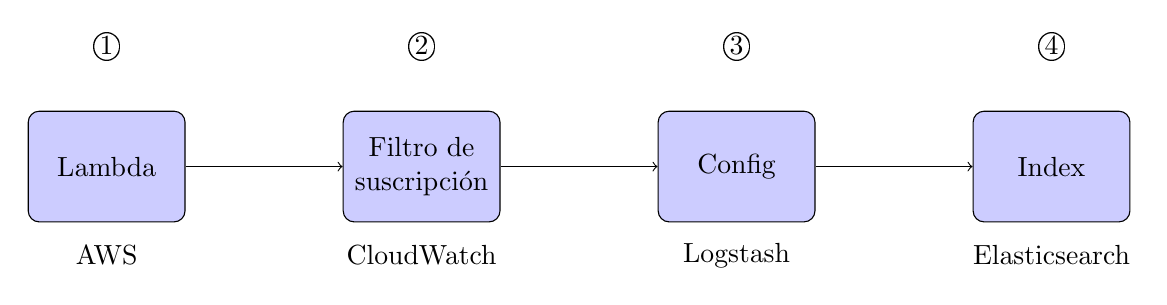
\begin{tikzpicture}[node distance=2cm, auto]
		% Definición de estilos
		\tikzstyle{block} = [rectangle, draw, fill=blue!20,
			text width=5em, text centered, rounded corners, minimum height=4em]
		\tikzstyle{line} = [draw, ->]

		% Nodos
		\node [block] (lambda) {Lambda};
		\node [block, right of=lambda, node distance=4cm] (filtro) {Filtro de suscripción};
		\node [block, right of=filtro, node distance=4cm] (logstash) {Config};
		\node [block, right of=logstash, node distance=4cm] (indice) {Index};

		% Conexiones
		\path [line] (lambda) -- (filtro);
		\path [line] (filtro) -- (logstash);
		\path [line] (logstash) -- (indice);

		% Etiquetas
		\node [below of=lambda, node distance=1.125cm] {AWS};
		\node [below of=filtro, node distance=1.125cm] {CloudWatch};
		\node [below of=logstash, node distance=1.125cm] {Logstash};
		\node [below of=indice, node distance=1.125cm] {Elasticsearch};

		\node [above of=lambda, node distance=1.5cm] {\textcircled{\raisebox{-0.9pt}{1}}};
		\node [above of=filtro, node distance=1.5cm] {\textcircled{\raisebox{-0.9pt}{2}}};
		\node [above of=logstash, node distance=1.5cm] {\textcircled{\raisebox{-0.9pt}{3}}};
		\node [above of=indice, node distance=1.5cm] {\textcircled{\raisebox{-0.9pt}{4}}};
	\end{tikzpicture}
	\caption{Proceso de ingesta de logs de balanceadores de carga de AWS}
	\label{fig:ingesta-logs-aws}
\end{figure}

El código completo de las cuatro partes se encuentra en el anexo \fullref{anexo:elb}.


\newpage{}
\subsection{Otros métodos de ingesta}\label{subsec:impl_ingesta_otros}
Pese a que el desarrollo y el alcance del proyecto se centra en la ingesta de
datos a través de Kafka, existen otras formas de ingestar datos en el stack
ELK, como por ejemplo:

\begin{itemize}
	\item \textbf{Beats:} Beats es una familia de agentes que se encargan de
		la recolección de datos y su envío a Elasticsearch. Existen diferentes
		tipos de Beats, como Metricbeat, Filebeat o Heartbeat, que se adaptan a
		diferentes necesidades. Todos ellos son compatibles con la arquitectura
		planteada y son alternativas válidas y atractivas para el futuro de la
		solución.
	\item \textbf{Conectores:} Elastic cuenta con conectores oficiales para
		diferentes aplicaciones de terceross comúnes, como Dropbox, Gmail o
		Jira. Estos conectores se encargan de la ingesta de datos de manera
		automática y son una opción a tener en cuenta.
	\item \textbf{Índices de API:} Elasticsearch permite la ingestión de datos
		a través de su API REST, lo que permite la integración con cualquier
		sistema que pueda enviar datos a través de HTTP.
	\item \textbf{Subida de ficheros:} A través de la interfaz de Kibana, es
		posible subir ficheros de datos para su ingestión en Elasticsearch. Esta
		opción es poco apropiada para el sistema planteado, pero puede resultar
		útil en caso de contar con información suelta de fuentes no habituales o
		para pruebas puntuales.
	\item \textbf{\textit{Web crawlers}:} una de las historias de usuario
		planteadas en la sección \fullref{sec:planif_inicial} es la ingesta de
		datos de webs de terceros. Elasticsearch cuenta con una funcionalidad
		diseñada con este objetivo, por lo que es una posibilidad clara.
\end{itemize}
